\documentclass[Screen16to9,17pt]{foils}
\usepackage{zencurity-slides}
\externaldocument{system-integration-exercises}
\selectlanguage{english}

\usepackage{tikz}
\usetikzlibrary{mindmap,trees}
\usetikzlibrary{shapes.geometric, arrows,automata}
\usetikzlibrary{positioning}

\tikzset{
    state/.style={
           rectangle,
           rounded corners,
           draw=black, very thick,
           minimum height=2em,
           inner sep=2pt,
           text centered,
           },
}



% Systemintegration

\begin{document}

\mytitlepage
{5. Using components, JMS
 databases}
{KEA System Integration F2020 10 ECTS}

\slide{Plan for today}

\begin{list2}
\item EIP book chapters
\item Using Camel components
\item Examples of FTP, JMS, Networking, Databases, timing and scheduling
 databases
\item Talk about protocols SMTP, IMAP, FTP, SFTP
\item Try some tools, find examples of applications
\end{list2}

Exercises
\begin{list2}
\item Running ActiveMQ
\item Camel book exercises
\item Discussions about application that use these components
\end{list2}



\slide{Reading Summary}

\begin{list1}
\item EIP Chapter 5 Message Construction
\item EIP Chapter 6 Simple Messaging
\item Camel chapter 6: Using components

\end{list1}



\slide{Todays Agenda - approximate time plan}

\begin{list2}
\item 08:30 45m Book chapters 5 and 6 discussion
\item 45m Chapter 5 Message Construction Chapter 6 Simple Messaging
\item 10:00 Break 15m
\item 10:15 45m Exercise: Active MQ
\item 45m 2x 45m Camebook chapter 6: Using components\\
 - contains
\item 11:45 Lunch Break
\item 12:30 Continued Camelbook chapter 6
\item 45m Exercise:
\item 14:00 Break 15m
\item 45m Investigate real-life examples
\end{list2}


\slide{Goals for today}

\hlkimage{6cm}{thomas-galler-hZ3uF1-z2Qc-unsplash.jpg}

Todays goals:
\begin{list2}
\item Know more integration patterns
\item See that Camel can be used for these patterns
\item Try ActiveMQ
\item Understand difference between SMTP submission, SMTP and IMAP
\end{list2}

Photo by Thomas Galler on Unsplash


\slide{Part 1-2: EIP Chapters 5 and 6}

Chapter 5 Message Construction



\slide{Message intent}


\begin{quote}
Message intent — Messages are ultimately just bundles of data, but the sender can have different intentions for what it expects the receiver to do with the message. It can send a Command Message, specifying a function or method on the receiver that the sender wishes to invoke. The sender is telling the receiver what code to run. It can send a Document Message, enabling the sender to transmit one of its data structures to the receiver. The sender is passing the data to the receiver, but not specifying what the receiver should necessarily do with it. Or it can send an Event Message, notifying the receiver of a change in the sender. The sender is not telling the receiver how to react, just providing notification.
\end{quote}
Source:  more or less same as the book\\{\footnotesize \url{https://www.enterpriseintegrationpatterns.com/patterns/messaging/MessagingChannelsIntro.html}}


\slide{Returning a response}


\begin{quote}
Returning a response — When an application sends a message, it often expects a response confirming that the message has been processed and providing the result. This is a Request-Reply scenario. The request is usually a Command Message, and the reply is a Document Message containing a result value or an exception. The requestor should specify a Return Address in the request to tell the replier what channel to use to transmit the reply. The requestor may have multiple requests in process, so the reply should contain a Correlation Identifier that specifies which request this reply corresponds to. [JMS11, pp.27-28]
\end{quote}
Source:  more or less same as the book\\{\footnotesize \url{https://www.enterpriseintegrationpatterns.com/patterns/messaging/MessagingChannelsIntro.html}}


\slide{Continued on the web site}

\begin{list2}
\item Message Construction\\{\footnotesize
\url{https://www.enterpriseintegrationpatterns.com/patterns/messaging/MessageConstructionIntro.html}}
\item Last part of chapter 5 includes Format Indicator\\{\footnotesize
\url{https://www.enterpriseintegrationpatterns.com/patterns/messaging/FormatIndicator.html}}
\end{list2}


\slide{Chapter 6 Simple Messaging}

\begin{list2}
\item Simple Message Examples\\{\footnotesize
\url{https://www.enterpriseintegrationpatterns.com/patterns/messaging/SimpleMessagingIntro.html}}
\end{list2}
\slide{Part 3: Exercise with JMS Example ActiveMQ}

\slide{Apache ActiveMQ}

\begin{quote}
Apache ActiveMQ™ is the most popular open source, multi-protocol, Java-based messaging server. It supports industry standard protocols so users get the benefits of client choices across a broad range of languages and platforms. Connectivity from C, C++, Python, .Net, and more is available. Integrate your multi-platform applications using the ubiquitous AMQP protocol. Exchange messages between your web applications using STOMP over websockets. Manage your IoT devices using MQTT. Support your existing JMS infrastructure and beyond. ActiveMQ offers the power and flexibility to support any messaging use-case.
\end{quote}

\url{https://activemq.apache.org/}

\exercise{ex:activemq-install}




\slide{Part 4-5: Camel book Chapter 6 Using components}

\slide{Camel Components}

\begin{quote}
Components are the primary extension point in Camel. Over the years since Camel’s
inception, the list of components has grown. As of version 2.20.1, Camel ships with
more than 280 components, and dozens more are available separately from other com-
munity sites.
\end{quote}
Source: \emph{Camel in action}, Claus Ibsen and Jonathan Anstey, 2018


\slide{Components chapter 6}

\hlkimage{17cm}{camelbook-6-0-components.png}

\slide{6.1 Overview of Camel components}

\hlkimage{13cm}{camelbook-6-1-component-class.png}

\begin{list2}
\item Manually adding components
\item Autodiscovering components
\end{list2}

\slide{Autodiscovering components}

\hlkimage{13cm}{camelbook-6-1-2-autodiscovery.png}

Autodiscovery is the way the components that ship with Camel are registered. To discover new components, Camel looks in the META-­INF/services/org/apache/camel/
component directory on the classpath for files. Files in this directory determine the
name of a component and the fully qualified class name.


\slide{6.2 Working with files: File and FTP components}

\hlkimage{20cm}{camelbook-6-2-files-ftp.png}

\begin{list2}
\item Reading and writing files with the File component,
\item Accessing remote files with the FTP component
\end{list2}

To see what happens firsthand, you can try the example by changing to the chapter6/file directory in the book’s source code and executing the following command:
\verb+mvn camel:run+

\slide{FTP File Transfer Protocol}

\begin{quote}
  The File Transfer Protocol (FTP) is a standard network protocol used for the transfer of computer files between a client and server on a computer network.

FTP is built on a client-server model architecture using separate control and data connections between the client and the server.[1] FTP users may authenticate themselves with a clear-text sign-in protocol, normally in the form of a username and password, but can connect anonymously if the server is configured to allow it. For secure transmission that protects the username and password, and encrypts the content, FTP is often secured with SSL/TLS (FTPS) or {\bf replaced with SSH File Transfer Protocol (SFTP)}.
\end{quote}

\url{https://en.wikipedia.org/wiki/File_Transfer_Protocol}

\slide{Camel FTP support}

Camel supports three flavors of FTP:
\begin{list2}
\item Plain FTP mode transfer
\item  Secure FTP (SFTP) for secure transfer
\item  FTP Secure (FTPS) for transfer with the Transport Layer Se
\end{list2}

The FTP component inherits all the features and options of the File component, and it
adds a few more options, as shown in table 6.4. For a complete listing of options for the
FTP component, see the online documentation (http://camel.apache.org/ftp2.html).

To run this example, change to the chapter6/ftp directory and run this command:
\verb+mvn camel:run+

Spring does not really want to work.


\slide{Java 8 on Debian 10/9/8}

\begin{quote}
How do I Install Java 8 on Debian?. The first Oracle Java 8 stable version was released on Mar 18, 2014, and available to download and install. Oracle Java PPA for Debian systems is being maintained by Webupd8 Team. JAVA 8 is released with many of new features and security updates. This tutorial will help you to Install Java 8 on Debian 9/8/7 systems using PPA and apt-get command.
\end{quote}

\url{https://tecadmin.net/install-java-8-on-debian/}

\slide{Install Java 8 on Debian}

\verb+sudo vim /etc/apt/sources.list.d/java-8-debian.list+
and add following content in it:
\begin{alltt}
deb http://ppa.launchpad.net/webupd8team/java/ubuntu trusty main
deb-src http://ppa.launchpad.net/webupd8team/java/ubuntu trusty main
\end{alltt}

Run the following to install
\begin{alltt}
sudo apt-key adv --keyserver keyserver.ubuntu.com --recv-keys EEA14886
sudo apt-get update
sudo apt-get install oracle-java8-installer
java -version
sudo apt-get install oracle-java8-set-default
\end{alltt}


\slide{6.3 Asynchronous messaging: JMS component}

\begin{list2}
\item Sending and receiving messages
\item Request-­reply messaging, Message mappings
\end{list2}

\slide{Camel with JMS}

Camel doesn’t ship with a JMS provider; you need to configure Camel to use a specific
JMS provider by passing in a ConnectionFactory instance. For example, to connect to
an Apache ActiveMQ broker listening on port 61616 of the local host, you could configure the JMS component like this:

\begin{minted}[fontsize=\footnotesize]{xml}
<bean id="jms" class="org.apache.camel.component.jms.JmsComponent">
<property name="connectionFactory">
<bean class="org.apache.activemq.ActiveMQConnectionFactory">
<property name="brokerURL" value="tcp://localhost:61616"/>
</bean>
</property>
</bean>
\end{minted}

The tcp://localhost:61616 URI passed in to ConnectionFactory is JMS provider-­
specific. In this example, you’re using the ActiveMQConnectionFactory , so the URI is
parsed by ActiveMQ. The URI tells ActiveMQ to connect to a broker by using TCP on
port 61616 of the local host.

\slide{Connection Pooling}

The ActiveMQ component\\
By default, a JMS ConnectionFactory doesn’t pool connections to the broker, so it
spins up new connections for every message. The way to avoid this is to use connection
factories that use connection pooling.

For convenience to Camel users, ActiveMQ ships with the ActiveMQ component, which
automatically configures connection pooling for improved performance. The ActiveMQ
component is used as follows:

\begin{minted}[fontsize=\footnotesize]{xml}
<bean id="activemq"
class="org.apache.activemq.camel.component.ActiveMQComponent">
<property name="brokerURL" value="tcp://localhost:61616"/>
</bean>
\end{minted}

Same can be found with database connections.

\slide{Request-reply messaging}

\hlkimage{23cm}{camelbook-6-3-2-request-reply.png}

Camel takes care of this style of messaging so you don’t have to create special reply
queues, correlate reply messages, and the like. By changing the message exchange pat-
tern (MEP) to InOut , Camel will enable request-­reply mode for JMS.

\slide{Message mappings: Sending to JMS}

\hlkimage{20cm}{camelbook-6-6-sending-jms.png}

\slide{Message mappings: Receive from JMS}

\hlkimage{20cm}{camelbook-6-7-receive-jms.png}

Note: To disable message mapping for body types, set the mapJmsMessage URI option to
\verb+false+ .


\slide{Header mapping}

Headers in JMS are even more restrictive than body types. In Camel, a header can be
named anything that will fit in a Java String , and its value can be any Java object. This
presents a few problems when sending to and receiving from JMS destinations.
These are the restrictions in JMS:
\begin{list2}
\item Header names that start with JMS are reserved; you can’t use these header names.
\item Header names must be valid Java identifiers.
\item Header values can be any primitive type and their corresponding object
types. These include boolean , byte , short , int , long , float , and double .
Valid object types include Boolean , Byte , Short , Integer , Long , Float , Double ,
and String .
\end{list2}

\vskip 2cm
\centerline{Great example of the conversion problems seen in system integration}

\slide{6.4 Networking: Netty4 component}

\begin{quote}
  Another essential mode of integration is using
low-­level networking protocols, such as the Transmission Control Protocol (TCP)
and the User Datagram Protocol (UDP). Even if you haven’t heard of these protocols
before, you’ve definitely used them—protocols such as email, FTP, and HTTP run on
top of TCP.

To communicate over these and other protocols, Camel uses Netty and Apache
MINA. Both Netty and MINA are networking frameworks that provide asynchronous
event-­driven APIs and communicate over various protocols including TCP and UDP.
In this section, we use Netty to demonstrate low-­level network communication with
Camel.
\end{quote}

\begin{list2}
\item Using Netty for network programming
\item Using custom codecs
\end{list2}

\slide{TCP server with Netty}

\hlkimage{20cm}{camelbook-6-4-1-netty-sensor.png}

In Camel, a possible solution is accomplished with a single line:
\begin{minted}[fontsize=\footnotesize]{java}
from("netty4:tcp://localhost:8999?textline=true&sync=false")
.to("jms:operations");
\end{minted}

Here you set up a TCP server on port 8999 by using Netty, and it parses messages
by using the textline codec. The sync property is set to false to make this route
InOnly —any clients sending a message won’t get a reply back.

\slide{Textline codec}


\hlkimage{18cm}{camelbook-6-4-1-netty-codec.png}

A codec decodes or encodes the message data into something that the applications
on either end of the communications link can understand. As figure 6.8 illustrates, the
textline codec is responsible for grabbing packets as they come in and trying to piece
together a message that’s terminated by a specified character.

This example is provided in the book’s source in the chapter6/netty directory. Try it by using the following command:
\verb+mvn test -Dtest=NettyTcpTest+

\slide{6.5 Working with databases: JDBC and JPA components}

\begin{list2}
\item Accessing data with the JDBC component
\item Persisting objects with the JPA component
\end{list2}

\slide{Using Persistence}

\hlkimage{13cm}{camelbook-5-5-fail-complete.png}

\slide{Camel database support}

In pretty much every enterprise-­level application, you need to integrate with a database at some point, so it makes sense that Camel has first-­class support for accessing databases. Camel has five components that let you access databases in various ways:
\begin{list2}
\item \emph{JDBC component} -- Allows you to access JDBC APIs from a Camel route.
item SQL component—Allows you to write SQL statements directly into the URI of the
component for using simple queries. This component can also be used for call-
ing stored procedures.
\item \emph{JPA component} -- Persists Java objects to a relational database by using the Java Persistence Architecture.
\item \emph{Hibernate component} -- Persists Java objects by using the Hibernate framework.
This component isn’t distributed with Apache Camel because of licensing
incompatibilities. You can find it at the camel-­extra project (https://github.
com/camel-­extra/camel-­extra).
\item \emph{MyBatis component} -- Allows you to map Java objects to relational databases.
\end{list2}


\slide{Hibernate framework}

\begin{quote}
  Hibernate ORM (or simply Hibernate) is an object-relational mapping tool for the Java programming language. It provides a framework for mapping an object-oriented domain model to a relational database. Hibernate handles object-relational impedance mismatch problems by replacing direct, persistent database accesses with high-level object handling functions.

  Hibernate is free software that is distributed under the GNU Lesser General Public License 2.1.

  Hibernate's primary feature is mapping from Java classes to database tables, and mapping from Java data types to SQL data types. Hibernate also provides data query and retrieval facilities. It generates SQL calls and relieves the developer from the manual handling and object conversion of the result set.
\end{quote}

\url{https://en.wikipedia.org/wiki/Hibernate_(framework)}

\slide{SQLite RDMBS}

\begin{quote}
  SQLite is a relational database management system (RDBMS) contained in a C library. In contrast to many other database management systems, SQLite is not a client–server database engine. Rather, it is embedded into the end program.

SQLite is ACID-compliant and implements most of the SQL standard, generally following PostgreSQL syntax. ...

SQLite is a popular choice as embedded database software for local/client storage in application software such as web browsers. It is arguably the most widely deployed database engine, as it is used today by several widespread browsers, operating systems, and embedded systems (such as mobile phones), among others.[8] SQLite has bindings to many programming languages.
\end{quote}

\url{https://en.wikipedia.org/wiki/SQLite}

Both Hibernate and SQLite are very popular


\slide{JMS to Database example}

\hlkimage{20cm}{camelbook-jdb-order.png}

\begin{minted}[fontsize=\footnotesize]{java}
from("jms:accounting")
.to("bean:orderToSql")
.to("jdbc:dataSource?useHeadersAsParameters=true");
\end{minted}

\slide{Uses a bean for mapping}

Listing 6.3   A bean that converts an incoming order to a SQL statement:
\begin{minted}[fontsize=\footnotesize]{java}
public class OrderToSqlBean {
    public String toSql(@XPath("order/@name") String name,
                        @XPath("order/@amount") int amount,
                        @XPath("order/@customer") String customer,
                        @Headers Map<String, Object> outHeaders) {
        outHeaders.put("partName", name);
        outHeaders.put("quantity", amount);
        outHeaders.put("customer", customer);
        return "insert into incoming_orders"
            + "(part_name, quantity, customer) values"
            + " (:?partName, :?quantity, :?customer)";
    }
}
\end{minted}

The last part is an SQL statement doing the \emph{inserting} into the database

\slide{6.6 In-­memory messaging: Direct, Direct-­VM, SEDA, and VM
components}

\begin{quote}
  Camel provides four main components in the core to handle in-­memory messaging.
For synchronous messaging, there are the Direct and Direct-­VM components. For asyn-
chronous messaging, there are the SEDA and VM components. The only difference
between Direct and Direct-­VM is that the Direct component can be used for communi-
cation within a single CamelContext , whereas the Direct-­VM component is a bit broader
and can be used for communication within a JVM.
\end{quote}

\begin{list2}
\item Synchronous messaging with Direct and Direct-­VM
\item Asynchronous messaging with SEDA and VM
\end{list2}

Advanced concept we won't go further into, staged event-­driven architecture (SEDA) is described on Wikipedia too \url{https://en.wikipedia.org/wiki/Staged_event-­driven_architecture}





\slide{6.7 Automating tasks: Scheduler and Quartz2 components}

\begin{quote}
  Often in enterprise projects you need to schedule tasks to occur either at a specified
  time or at regular intervals. Camel supports this kind of service with the Timer, Sched-
  uler, and Quartz2 components. The Scheduler component is useful for simple recur-
  ring tasks, but when you need more control of when things get started, the Quartz2
  component is a must. The Timer component can also be used for simple recurring
  tasks. The difference is the Scheduler component uses the improved Java scheduler
  API, as opposed to the Timer component which uses the older java.util.Timer API.
\end{quote}

\begin{list2}
\item Using the Scheduler component
\item Enterprise scheduling with Quartz 231
\end{list2}

\slide{Lets try them}


You can run this simple example by changing to the chapter6/scheduler directory of
the book’s source and running this command:
\verb+mvn test -Dtest=SchedulerTest+

You can run this simple example by changing to the chapter6/quartz directory of
the book’s source and running this command:
\verb+mvn test -Dtest=QuartzTest+

To try an example using a cron trigger, browse to the chapter6/quartz directory and
run the QuartzCronTest test case with this Maven command:
\verb+mvn test -Dtest=QuartzCronTest+

\vskip 2cm
\centerline{Make changes and rerun the examples also}


\slide{6.8 Working with email}

Camel provides several components to work with email:
\begin{list2}
\item Mail component—This is the primary component for sending and receiving email
in Camel.
\item  AWS-­SES component—Allows you to send email by using the Amazon Simple Email
Service (SES).
\item GoogleMail component—Gives you access to Gmail via the Google Mail Web API.
\end{list2}


\begin{list2}
\item Sending mail with SMTP
\item  Receiving mail with IMAP
\end{list2}


\slide{SMTP Simple Mail Transfer Protocol}

\begin{quote}
  The Simple Mail Transfer Protocol (SMTP) is a communication protocol for electronic mail transmission. As an Internet standard, SMTP was first defined in 1982 by RFC 821, and updated in 2008 by RFC 5321 to Extended SMTP additions, which is the protocol variety in widespread use today. Mail servers and other message transfer agents use SMTP to send and receive mail messages.
\end{quote}

\url{https://en.wikipedia.org/wiki/Simple_Mail_Transfer_Protocol}

\slide{Camel SMTP}

Whenever you send an email, you’re using the Simple Mail Transfer Protocol (SMTP)
under the hood. In Camel, an SMTP URI looks like this:
\verb+[smtp|stmps]://[username@]host[:port][?options]+

\hlkimage{16cm}{camelbook-6-8-camel-smtp.png}

SMTP should always be protected with password!

\slide{Postfix}

\hlkimage{3cm}{postfix-mouse.png}

\begin{quote}
  Postfix is a free and open-source mail transfer agent (MTA) that routes and delivers electronic mail.

It is released under the IBM Public License 1.0 which is a free software license. Alternatively, starting with version 3.2.5, it is available under the Eclipse Public License 2.0 at the user's option.[2]

Originally written in 1997 by Wietse Venema at the IBM Thomas J. Watson Research Center in New York, and first released in December 1998[3], Postfix continues as of 2020 to be actively developed by its creator and other contributors.
\end{quote}
Source: \url{https://en.wikipedia.org/wiki/Postfix_(software)}

Home page: \url{http://www.postfix.org/}


\slide{Dovecot}

\begin{quote}
Dovecot is an open-source IMAP and POP3 server for Unix-like operating systems, written primarily with security in mind.[3] Timo Sirainen originated Dovecot and first released it in July 2002. Dovecot developers primarily aim to produce a lightweight, fast and easy-to-set-up open-source email server.

The primary purpose of Dovecot is to act as mail storage server. Mail is delivered to the server using some mail delivery agent (MDA) and stored for later access with an email client (mail user agent, or MUA).
\end{quote}
Source: \url{https://en.wikipedia.org/wiki/Dovecot_(software)}

\begin{quote}
Dovecot is an open source IMAP and POP3 email server for Linux/UNIX-like systems, written with security primarily in mind. Dovecot is an excellent choice for both small and large installations. It's fast, simple to set up, requires no special administration and it uses very little memory.
\end{quote}
Home page: \url{https://www.dovecot.org/}

\slide{Example of SMTP and IMAP}

\begin{center}
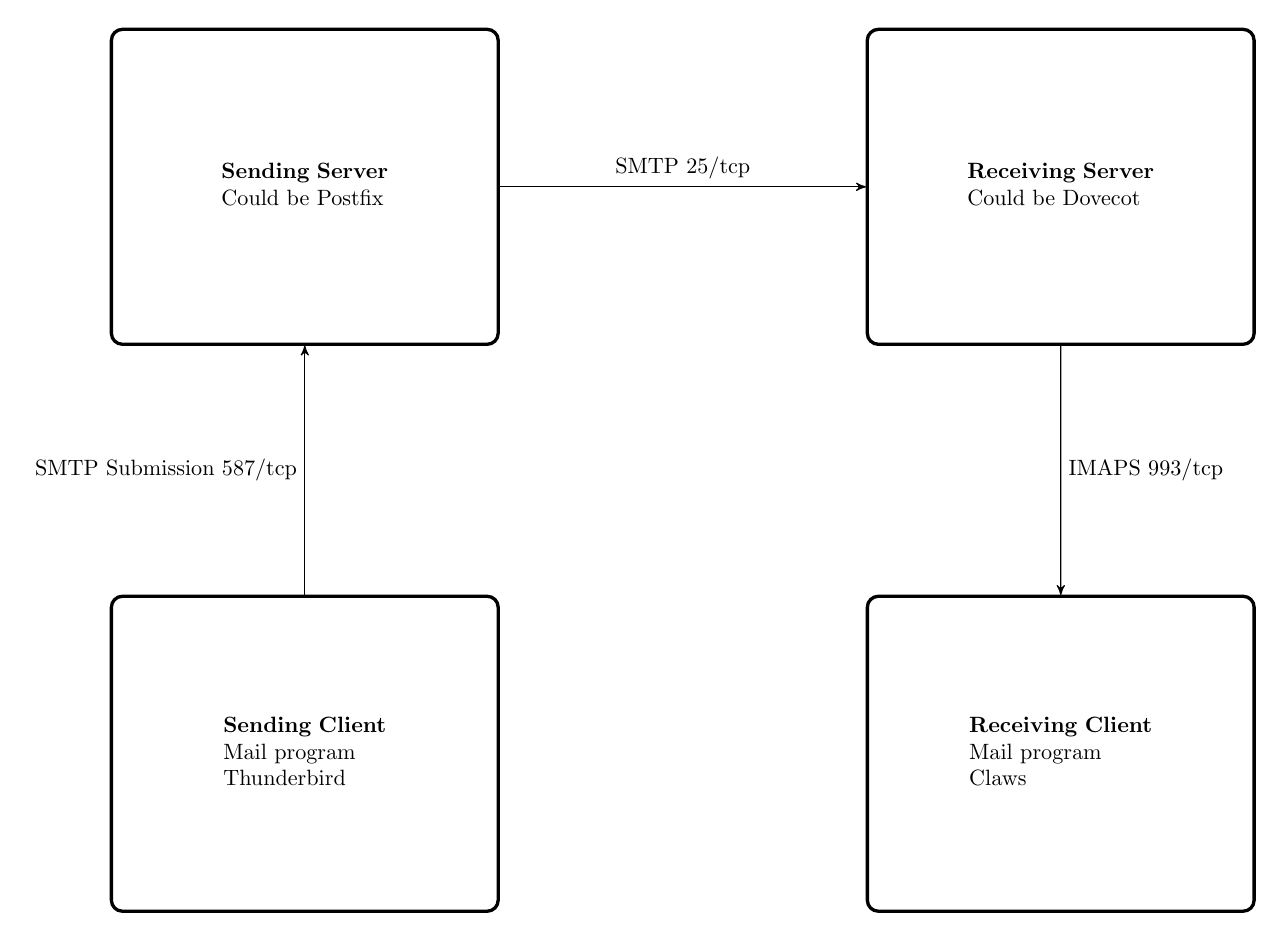
\begin{tikzpicture}[->,>=stealth',scale=0.8, transform shape]
  \newlength{\boxwidth}
  \setlength{\boxwidth}{6cm}
  \newlength{\boxheight}
  \setlength{\boxheight}{5cm}
  \newlength{\boxspace}
  \setlength{\boxspace}{12cm}

  % http://texample.net/tikz/examples/epc-flow-charts/

  % https://www.overleaf.com/learn/latex/LaTeX_Graphics_using_TikZ:_A_Tutorial_for_Beginners_(Part_3)%E2%80%94Creating_Flowcharts

   % Use previously defined 'state' as layout (see above)
   % use tabular for content to get columns/rows
   % parbox to limit width of the listing
   \node[state,text width=\boxwidth,minimum height=\boxheight] (SENDER)
   {\begin{tabular}{l}
   {\bf Sending Server}\\
      Could be Postfix
   \end{tabular}};

   %
   \node[state,    	% layout (defined above)
    text width=\boxwidth, 	% max text width
    minimum height=\boxheight,
    %yshift=2cm, 		% move 2cm in y
    right of=SENDER, 	% Position is to the right of QUERY
    node distance=\boxspace, 	% distance to First node
    anchor=center] (RECEIVER) 	% posistion relative to the center of the 'box'
   {%
   \begin{tabular}{l}
   {\bf Receiving Server}\\
Could be Dovecot
   \end{tabular}};

   \node[state,
    below of=SENDER,
    yshift=-8cm,
    anchor=center,
    minimum height=\boxheight,
    text width=\boxwidth] (THUNDERBIRD)
   {%
   \begin{tabular}{l}
   {\bf Sending Client}\\
    Mail program\\
    Thunderbird
   \end{tabular}
   };

   \node[state,
    below of=RECEIVER,
    yshift=-8cm,
    anchor=center,
    minimum height=\boxheight,
    text width=\boxwidth] (CLAWS)
   {%
   \begin{tabular}{l}
   {\bf Receiving Client}\\
    Mail program\\
    Claws
   \end{tabular}
   };

   % draw the paths and and print some Text below/above the graph
   \path
   (SENDER) 	edge node[anchor=north,above]{SMTP 25/tcp} (RECEIVER)
   (THUNDERBIRD) 	edge node[anchor=west,left]{SMTP Submission 587/tcp} (SENDER)
   (RECEIVER) edge node[anchor=east,right]{IMAPS 993/tcp }   (CLAWS);

\end{tikzpicture}
\end{center}




\slide{6.9 Summary and best practices}


The Camel website has documentation on all components available -- We could cover
only the most widely used and important components in this book, so if you need
to use one of the many other components, documentation is available at
\url{http://camel.apache.org/components.html}.

\slide{Part 6: Run application which incorporates system integration}

A lot of applications are running ActiveMQ inside. A list is available on the web page:\\
\url{http://activemq.apache.org/projects-using-activemq}

There are also alternatives to ActiveMQ, one such is RabbitMQ.


\slide{RabbitMQ}

\begin{quote}
RabbitMQ is an open-source message-broker software (sometimes called message-oriented middleware) that originally implemented the Advanced Message Queuing Protocol (AMQP) and has since been extended with a plug-in architecture to support Streaming Text Oriented Messaging Protocol (STOMP), Message Queuing Telemetry Transport (MQTT), and other protocols.[1]

The RabbitMQ server program is written in the Erlang programming language and is built on the Open Telecom Platform framework for clustering and failover. Client libraries to interface with the broker are available for all major programming languages.
\end{quote}

Source: \url{https://en.wikipedia.org/wiki/RabbitMQ}

Home page: \url{https://www.rabbitmq.com/}


\slide{Example from RabbitMQ tutorial: Sending}

Sending\\
The following code fragment establishes a connection, makes sure the recipient queue exists, then sends a message and finally closes the connection.

\inputminted[fontsize=\footnotesize]{python}{programs/sender.py}

Example from: \url{https://www.rabbitmq.com/tutorials/tutorial-one-python.html}

\slide{Example from RabbitMQ tutorial: Receiving}

Receiving\\
Similarly, the following program receives messages from the queue and prints them on the screen:

\inputminted[fontsize=\footnotesize]{python}{programs/recv.py}

\exercise{ex:rabbitmq-install}


\slide{Part 7: Do some research}

{\bf Investigate real-life examples}

Discussions about application that use these components

Find applications using Messages

1) Popular app, does Twitter use messaging?

2) One commercial application using or providing messaging

3) One Open Source application using or providing messaging



\slidenext

\end{document}
